
\frame[t] {
\frametitle{Pitman Yor Process (PYP) : Definition \cite{Pitman1997a}}
 A Pitman-Yor process $\PY(c,d,H)$ is a distribution over distributions with three parameters:
\begin{itemize}
\item A discount $ 0 \le d < 1 $ that controls power-law behavior
\begin{itemize}
\item $d=0$ is DP
\end{itemize}
\item A concentration $c > -d$ like that of the DP
\item A base distribution $H$ also like that of the DP
\end{itemize}
A draw $G \sim PY(c,d,H)$ is also atomic

\[G = \sum_{k=1}^{\infty} \pi_k \delta_{\phi_k}\].  
}

\frame[t]{
\frametitle{PYP: Stick-Breaking Construction}
The procedure for generating a draw from a PYP is to draw $\pi_k$ from a generalized stick-breaking procedure and $\phi_k$ as usual:
\[
\begin{array}{rcll}
\beta_k  & \sim & \Bet(1-d, c+kd) & \forall \, k = 1 \ldots \infty \\
&&& \\
\pi_k & = &  \beta_k \prod_{i=1}^{k-1}(1- \beta_i) & \forall \, k = 1 \ldots \infty \\
&&& \\
\phi_k  & \sim &  H & \forall \, k = 1 \ldots \infty
\end{array}
\]

The expected length of a stick $\mathbb{E}[\pi_k]$ falls off as a power law for large $k$ when $d \ne 0$.  When $d = 0$ the stick lengths fall off exponentially, and the PYP reduces to a Dirichlet process.
%The expected length of a stick is $\mathbb{E}[\pi_k] = \mathbb{E}[\beta_k]\prod_{i=1}^{k-1}(1 - \mathbb{E}[\beta_i]) = \frac{1-d}{1+c+(k-1)d}\prod_{i=1}^{k-1}\frac{c+id}{1+c+(i-1)d} = d(1-d)\frac{\Gamma(\frac{c}{d} + (k-1))}{\Gamma(\frac{c}{d})}\frac{\Gamma(\frac{1+c}{d})}{\Gamma(\frac{1+c}{d} + k)}$
}

\frame[t] {
\frametitle{PYP: Power Law}
\begin{figure}[t]
\begin{center}
%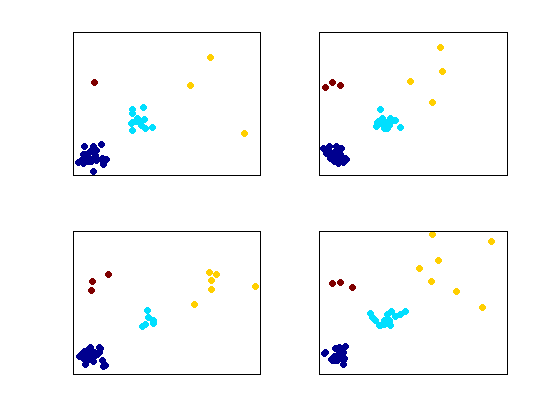
\includegraphics[trim = 4cm 8cm 4cm 8cm, clip, width=5cm]{fig/shared_clustering.pdf}
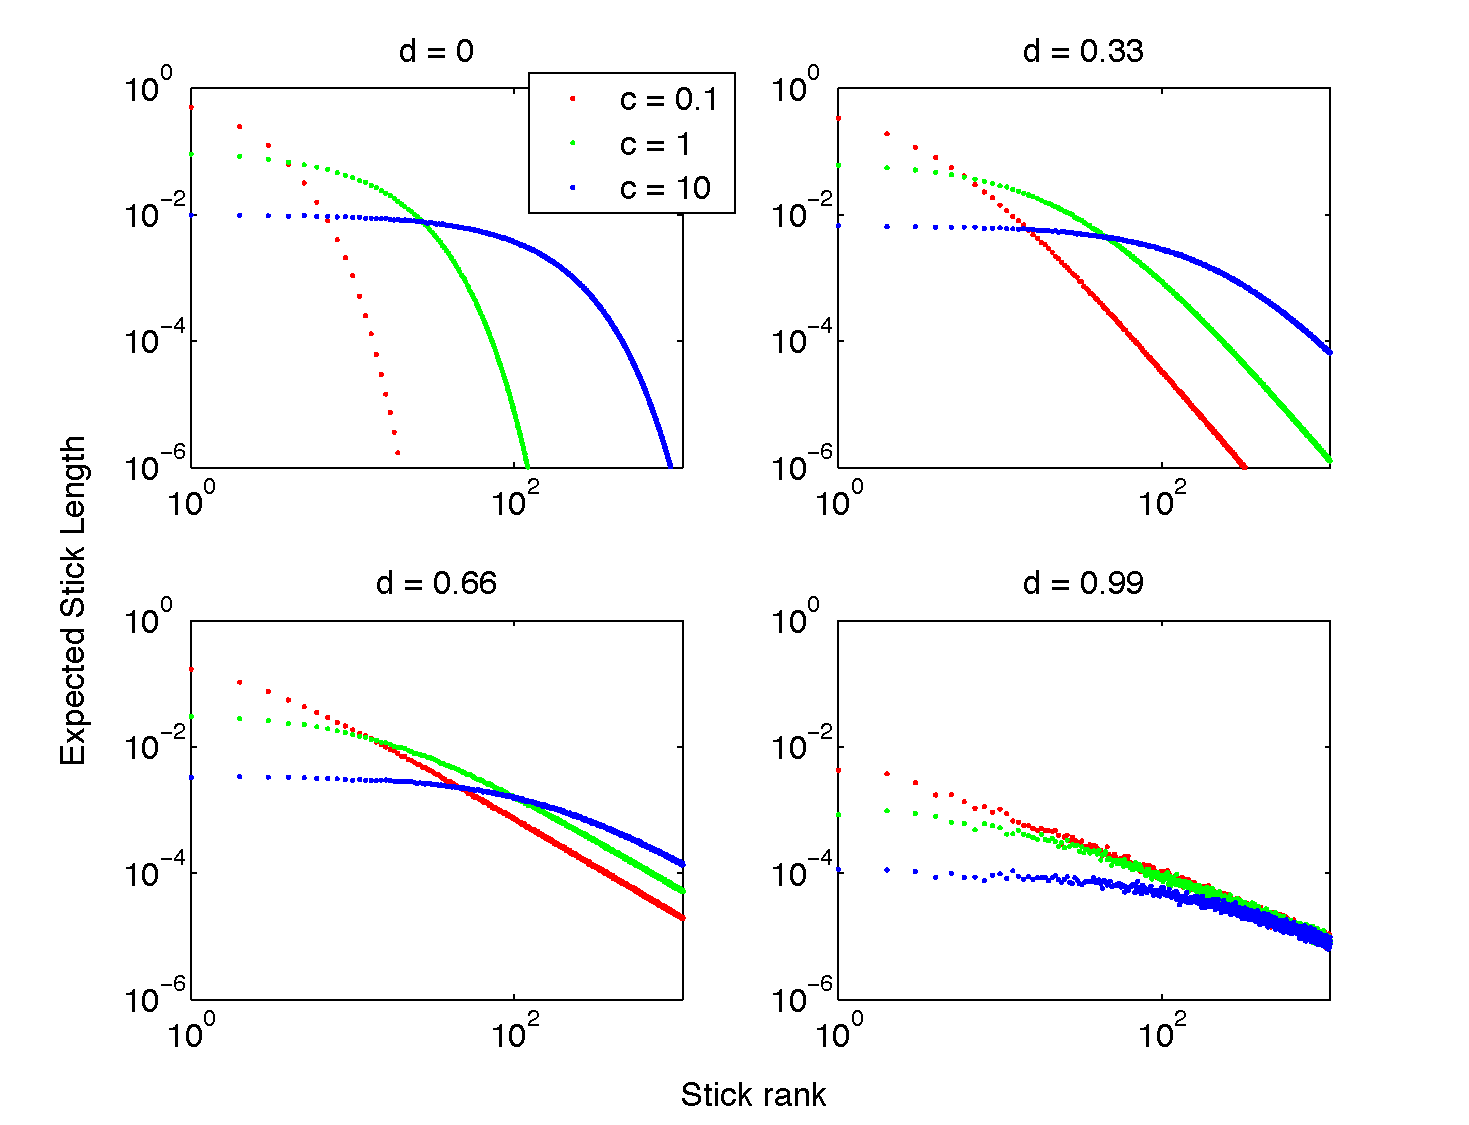
\includegraphics[width=8cm]{jtfig/pypl.pdf}
%\caption{Shared clustering}
\label{default}
\end{center}
\end{figure}
}

\frame[t] {
\frametitle{PYP: Polya Urn Representation}
As in the DP, the PYP posterior predictive distribution can be expressed with $G$ marginalized out.  
\begin{eqnarray*}
p(x_{n+1} | x_{1}, \ldots, x_n) & = & \Ave\left[\frac{m_k - d}{c+n}\delta(\phi_k-\cdot) + \frac{c + Kd}{c + n}H(\cdot)\right]
\end{eqnarray*}

This again forms the basis for similar SMC and MCMC inference algorithms.
\bigskip

Note: As in the case of the DP, due to the discrete nature of distributions $G \sim \PY(c,d,H)$, draws from $G$ tend to take the same value or ``cluster.''  
}

\frame[t] {
\frametitle{Hierarchical Pitman-Yor Process \cite{Teh2006a}}
A hierarchical Pitman-Yor process is the ``obvious'' two-parameter extension of the hierarchical Dirichlet process \cite{Teh2006b,Goldwater2006}.\\
\bigskip

Example:
%\begin{columns}[t]
%\begin{column}{.75\textwidth}
\begin{eqnarray*}
	\G_{[]} | \U_{\Sigma}, d_0 &\sim& \PY(d_0, 0, \U_{\Sigma }) \\
	\G_{\bf{u}} | \G_{\sigma(\bf{u})}, d_{|\bf{u}|} &\sim& \PY(d_{|\bf{u}|}, 0, \G_{\sigma(\bf{u})}) \hspace{.35cm} \forall {\bf u} \in \Sigma^+\\
	x_n | x_{n-1},  \ldots, x_1 = \bf{u} &\sim& \G_{\bf{u}}
\end{eqnarray*}
%\end{column}
%\begin{column}{.25\textwidth}
%\includegraphics[trim = 4cm 8cm 4cm 8cm, clip, width=5cm]{../../2010_icml/fig/sm_graphical_model.pdf}
%\todo{insert graphical model fig}
%\end{column}
%\end{columns}
%\bigskip
Estimation and inference follow that for the hierarchical Dirichlet process
}

\frame[t] {
\frametitle{Review}
\begin{block}{Summary}
\begin{itemize}
\item DP and PYP are flexible priors on distributions
\item Can think of either as glue for tying together related distributions in hierarchical models.
\item 
\end{itemize}
\end{block}
}